% RENDERING PREVIEW of ofc-qot.tex (digital-twin freshness reframe) in the standard
% article class, for PDF/DOCX deliverables. The OFFICIAL OFC submission uses the
% Optica opticameet3 class (Overleaf). Content identical to ../ofc-qot.tex.
\documentclass[10pt,twocolumn]{article}
\usepackage[letterpaper,margin=0.75in]{geometry}
\usepackage{mathptmx}
\usepackage{amsmath,amssymb}
\usepackage{graphicx}
\usepackage{caption}
\captionsetup{font=small,labelfont=bf}
\usepackage[colorlinks=true,citecolor=blue,urlcolor=blue,linkcolor=blue]{hyperref}
\setlength{\parindent}{1em}
\pagestyle{empty}

\title{\vspace{-2em}\textbf{How Stale Can an Optical Digital Twin Be?\\
A Measured Freshness Budget for QoT Decisions}}
\author{Andrew H. Bond\\
\small Department of Computer Engineering, San Jos\'e State University, San Jos\'e, CA 95192, USA\\
\small andrew.bond@sjsu.edu}
\date{}

\begin{document}
\twocolumn[
  \begin{@twocolumnfalse}
  \maketitle
  \begin{center}\begin{minipage}{0.86\textwidth}
  {\small\itshape \textbf{Rendering preview} (standard article class). The official OFC 2027
  submission is typeset with the Optica \texttt{opticameet3} meeting class; this document
  reproduces the identical content and figures. Every number is sealed and graded or
  deterministic.\par}
  \medskip

  \noindent\textbf{Abstract:} A GNPy-class digital twin makes format decisions between telemetry syncs while the
network fills. We measure the failure curve: false-clears are zero through four
channel adds, then cross a 5\% risk target near eight.
  \end{minipage}\end{center}
  \vspace{1.2em}
  \end{@twocolumnfalse}
]

\section{Introduction}
Digital twins of the optical physical layer are moving from research to
practice~\cite{dtwin}. A twin holds a QoT model of the deployed network, and
operators use it to answer provisioning questions: which format will this lightpath
sustain, how much margin does it need. The twin's answer is only as good as its view
of the network, and the view goes stale. Between telemetry syncs, channels are added,
nonlinear interference grows, and the GSNR the twin believes is no longer the GSNR
the receiver sees. The question every deployment must answer is how often the twin
needs to sync. Today that answer is set by engineering judgment. This paper gives it
a measured number.

We treat each twin decision as a certificate. The twin clears a format for a
lightpath, and the certificate fails when the deployed channel cannot support that
format. We call this failure a false-clear, and we measure its rate on the GN-model
physical layer of GNPy~\cite{gnpy} over the CORONET-CONUS reference network, with
fill statistics drawn from a public demand matrix. Three results follow. The
false-clear rate of a stale twin is zero until a few channels have been added to
the band a service shares along its path, then climbs steeply, crossing a $5\%$
risk target at about eight such adds: the twin's freshness budget. Which services
are exposed when the twin is stale is set by spectral position and reach, so a
per-lightpath view recovers real capacity over a uniform margin. And when the
twin's QoT model is a learned surrogate, training it on average error leaves it
blind exactly at the FEC threshold where its decisions are made.

\section{Method}
\textbf{Substrate.} Lightpaths are transparent shortest-path routes of the
CORONET-CONUS reference topology; per-channel GSNR comes from the GN model in
GNPy~\cite{gnpy}. Table~\ref{tab:subst} lists the parameters. The twin's view is
the band as last synced. The staleness variable $N$ is the number of channels
present in the C-band that co-propagates with the service along its own path (its
interference neighbourhood), and $\Delta N$ counts the channels added to that band
since the sync. $N$ runs from a lightly filled provisioning band of 6 to a full
grid of 76. The filling protocol is fixed and disclosed: the band fills as a
contiguous comb of 32\,GBd channels on the 50\,GHz grid, from the low-frequency
edge of the C-band ($191.35$\,THz) upward, so an add always lands at the top of
the comb. Each sweep point evaluates the certificate over 40 spectral positions
per fill level, across the route pool's span-count classes weighted by route
multiplicity. A certificate selects the highest of five declared formats whose
required GSNR the twin's estimate clears: QPSK, 8QAM, 16QAM, 32QAM and 64QAM at
$6.5$, $9.0$, $12.5$, $16.0$ and $19.0$\,dB respectively ($32$\,GBd, roughly
$20\%$-overhead soft-decision FEC; declared values, no probabilistic shaping). The
capacity result of \S\ref{sec:exposed} uses a rate-flexible transceiver instead:
spectral efficiency $\min(6,\log_2(1+\mathrm{SNR}/\Gamma))$ per polarisation with a
$\Gamma=1$\,dB gap for FEC and implementation.

\begin{table}[t]
\caption{Substrate parameters}
\label{tab:subst}
\centering
\footnotesize
\begin{tabular}{ll}
\hline
Topology & CORONET-CONUS (75 nodes; routes $\le 2500$\,km, 2--31 spans) \\
Fibre & SSMF, 0.2\,dB/km, $D=17$\,ps/nm/km, 80\,km spans \\
Amplifiers & EDFA, NF 6\,dB \\
Launch power & $+2$\,dBm per channel, flat (not re-optimised per fill) \\
Grid & 32\,GBd on 50\,GHz, C-band of 76 channels \\
QoT engine & GNPy GN model (analytic NLI) \\
Deployed fill & sampled from SNDlib janos-us-ca per-link distribution \\
Estimator noise & 0.3\,dB monitoring; 0.5\,dB RMSE in \S\ref{sec:exposed} \\
\hline
\end{tabular}
\end{table}

\textbf{Certificate, consumer, witness.} A certificate selects the highest format
whose required GSNR the twin's estimate clears. The consumer is that decision. The
witness is the true deployed GSNR, in practice the receiver's pre-FEC BER. For the
surrogate study the features are the synced GSNR plus spectral position, reach and
fill, the label carries an irreducible term for unmeasured network state, and two
gradient-boosted objectives compete: average-error (squared loss) and
decision-aware (a conservative quantile loss). Bars and manipulation checks are
pre-registered. The sealed record is content-hashed and graded on seeds disjoint
from those used during design~\cite{otcampaigns}.

\section{Results}
\subsection{The freshness budget}
The risk of a stale twin is driven by the fill added since its last sync. Sweeping
the deployed band from 6 to 76 channels while the twin's view stays at the sync
point gives the failure curve directly, and we report the curve rather than a fit.
The false-clear rate is zero through the first four added channels, crosses a
$5\%$ risk target at $8.1$ adds (interpolated between measured points), reaches
about $0.21$ by eighteen adds, and saturates near $0.5$ as the band fills. An
earlier draft summarised this as a linear law; the curve's flat onset and its
saturation make that the wrong summary, and review caught it. The measurement
stands as a curve, and the budget is its crossing: about eight added channels at
a $5\%$ risk target. The rule is concrete. Re-sync the twin, or re-certify the
affected services, before the band around them grows by about eight channels,
rather than on a fixed calendar. Given an arrival rate the budget converts to
time. A band taking one add per week can hold a sync for about two months. A busy
one taking one add per day must sync roughly weekly.

\subsection{Who is exposed when the twin is stale}
\label{sec:exposed}
Staleness does not spread its damage evenly. A lightpath's GSNR drops as neighbours
arrive, and whether it crosses a format threshold depends on where it sits:
false-clears concentrate on services whose spectral position and reach leave their
GSNR near a boundary, and are absent elsewhere (Fig.~\ref{fig:fc}). So a single
blanket margin cannot protect the fleet efficiently. We price this against today's
practice of one uniform system margin, with fill statistics grounded on public
demand data. Routing the 1482 demands of the SNDlib janos-us-ca reference
matrix~\cite{sndlib} (39 nodes, 61 undirected links) gives a per-link
channel-fill distribution with median 10 and 90th percentile 35 of 76; each
CORONET lightpath's deployed fill is then sampled independently from that
marginal distribution. The demand data grounds the fill statistics, not a routed
traffic snapshot: correlations between links along a route are not carried over.
What matters for the comparison is the heavy tail, which is exactly what a
marginal preserves: a uniform margin sized for the few near-full links
over-provisions the lightly filled majority. Giving both
policies the same estimator uncertainty of $0.5$\,dB RMSE, a twin that sizes each
margin to the lightpath's own fill recovers about $8\%$ of spectral efficiency, near
$0.33$\,b/sym or $21$\,Gb/s per channel, at matched safety (false-clear at most
$0.01$) on a rate-flexible transceiver model. The gain is capacity the uniform
margin strands on links that never fill.

\begin{figure}[t]
  \centering
  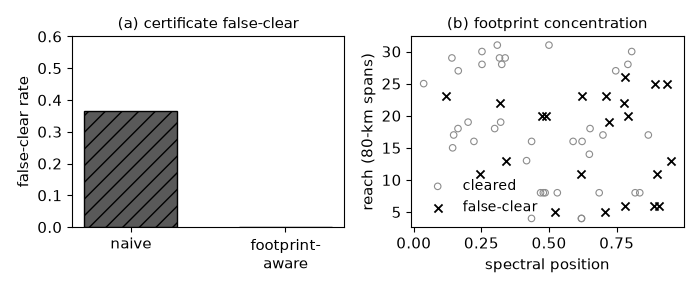
\includegraphics[width=\linewidth]{fc_footprint.png}
  \caption{Where a stale twin fails (GNPy over CORONET-CONUS). Per-service
  false-clear over spectral position and reach concentrates on threshold-adjacent
  services. A per-lightpath view removes it. Marker shape distinguishes classes.}
  \label{fig:fc}
\end{figure}

\subsection{The learned surrogate fails at the threshold}
Many twins replace the physics model with a learned surrogate for speed. How that
surrogate is trained matters more than how accurate it is on average.
Uncertainty-aware and quantile QoT models are established~\cite{quantileqot}; what
has not been measured is the price of ignoring them at the decision boundary. Under
irreducible prediction uncertainty the average-error surrogate wins the metric it
was trained on and loses the one the twin exists for. Its MAE is $0.65$\,dB against
$0.95$\,dB for the quantile objective, yet its false-clear rate is about $0.041$
against $0.008$, five times higher, at comparable delivered spectral efficiency near
$3.9$\,bits/symbol (Fig.~\ref{fig:ml}a). The failures sit where the true GSNR lies
within about a decibel below the \emph{next} format's threshold
(Fig.~\ref{fig:ml}b): there a small upward prediction error clears one format too
high, and nowhere else can it. That is the cliff, and a symmetric error metric is
blind there. A uniform backoff is the fair baseline and we report it: on the sealed
per-prediction records, backing the average-error surrogate off by a further
$0.85$\,dB matches the quantile model's false-clear at the same delivered bits. But
that $0.85$\,dB is found by tuning against witnessed outcomes after the fact; the
quantile objective reaches the same operating point from its training loss alone,
with no post-hoc knob, and the machinery to do so already
exists~\cite{quantileqot}.

\begin{figure}[t]
  \centering
  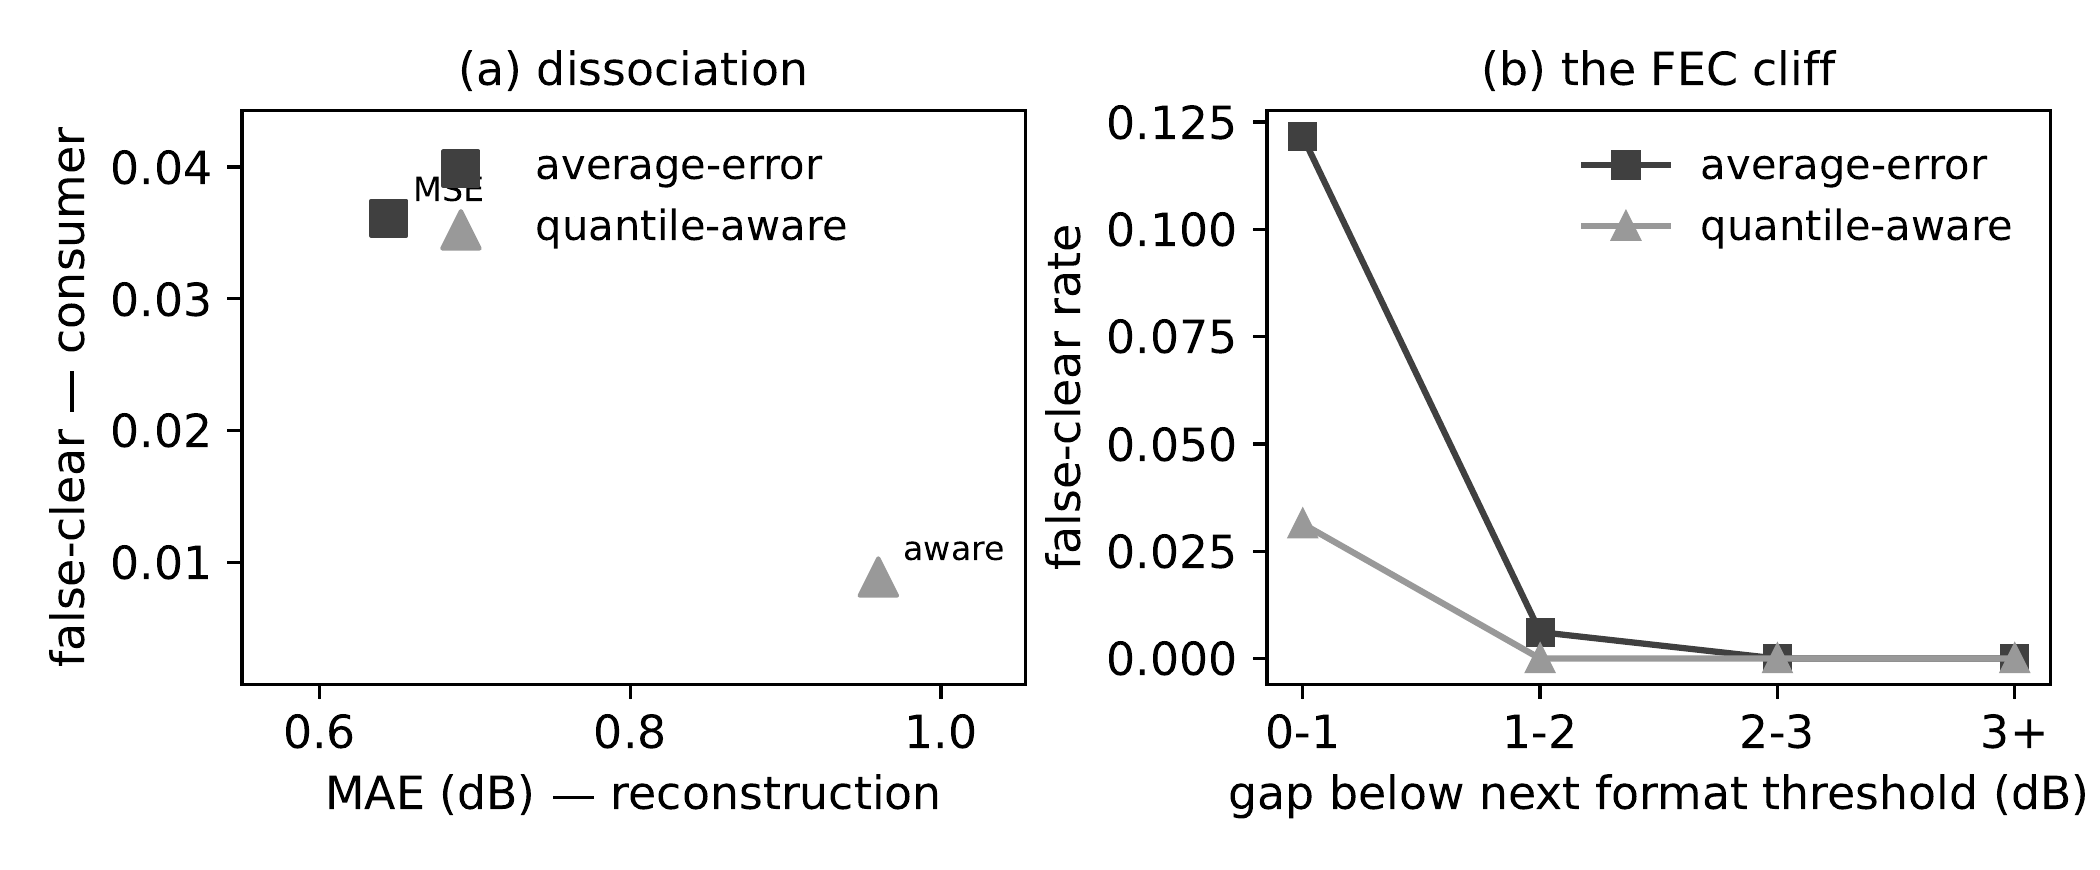
\includegraphics[width=\linewidth]{ml_cliff.png}
  \caption{Two surrogate objectives, two metrics (GNPy, gradient-boosted
  regressors). (a) The average-error objective has lower MAE and higher false-clear
  than the quantile objective. (b) Its false-clears concentrate where the true GSNR
  sits within a decibel below the next format threshold; services already clearing
  the top format cannot false-clear and are excluded. Marker shape distinguishes
  objectives.}
  \label{fig:ml}
\end{figure}

\section{Related work}
Optical digital twins are an active area, from GNPy-based twins fed by network
telemetry~\cite{dtwin} to calibration against field data; that work builds and
tunes the twin, and does not quantify how stale it can afford to be. Margin erosion
under channel add is known qualitatively, and impairment-aware provisioning
accounts for it at setup time~\cite{pointon}; our contribution is the measured
staleness law and the budget it implies for the twin that persists after setup.
Uncertainty-aware ML-QoT, including quantile models, is
established~\cite{quantileqot,mlqot}; we credit it as the correction for the
surrogate result and add the measured cliff dissociation that motivates it. We do
not offer a better twin, estimator or allocator. We offer the freshness budget, the
exposure map, and the price of the wrong training objective.

\section{Discussion}
A digital twin is a certificate factory, and certificates age. The freshness budget
turns twin synchronization from a judgment call into a provisioned quantity:
re-sync within eight adds to a service's band at a $5\%$ risk target, protect the
threshold-adjacent services first, and train surrogates on the decision rather than
the average. The evidence stands on the GN model with public demand data, and its
limits are worth stating. Launch power is flat at $+2$\,dBm and not re-optimised as
the band fills, ROADM filtering penalties are not modelled, and the witness is the
GN-model GSNR rather than a receiver's pre-FEC BER. These effects do not all push
the budget the same way: re-optimising launch power as the band fills would offset
part of the drop the twin misses, while filtering penalties would add to it. The
budget should be re-measured, not extrapolated, and a coherent-receiver witness on
a testbed twin is the natural next step. In companion sealed experiments, two
margin policies with equal fleet budgets received opposite verdicts from two
service classes whose failures ride different axes of the network state (cells
XPROTO-QOT-FLIP and XPROTO-CSI-FLIP in the sealed
repository~\cite{otcampaigns}); a full treatment of that inversion is beyond this
paper's scope and is reported separately. The same consumer-relative failure
appears in radio link adaptation and in database
replication~\cite{otcampaigns}. The results here stand on the optical QoT
certificate alone.

\begin{thebibliography}{9}
\small
\bibitem{gnpy} A.~Ferrari \emph{et al.}, ``GNPy: an open source application for
physical layer aware open optical networks,'' J.\ Opt.\ Commun.\ Netw.\ \textbf{12},
C31--C40 (2020).
\bibitem{dtwin} S.~Shen \emph{et al.}, ``End-to-end QoT predictions enhanced by
GNPy-based digital twin with network telemetry,'' in \emph{Proc. OFC}, Th2A.16
(2024). % authors verified 2026-08-26 (Univ. Bristol; was misattributed)
\bibitem{quantileqot} H.~Maryam, T.~Panayiotou, and G.~Ellinas, ``Learning
quantile QoT models to address uncertainty over unseen lightpaths,'' Comput.\
Netw.\ \textbf{212}, art.\ 108992 (2022). % verified 2026-08-26
\bibitem{mlqot} C.~Rottondi \emph{et al.}, ``Machine-learning method for quality of
transmission prediction of unestablished lightpaths,'' J.\ Opt.\ Commun.\ Netw.\
\textbf{10}, A286--A297 (2018). % verify vol/pages on final
\bibitem{pointon} Y.~Pointurier, ``Design of low-margin optical networks,'' J.\ Opt.\
Commun.\ Netw.\ \textbf{9}, A9--A17 (2017). % verify vol/pages on final
\bibitem{sndlib} S.~Orlowski, R.~Wess\"aly, M.~Pi\'oro, and A.~Tomaszewski,
``SNDlib 1.0---Survivable Network Design Library,'' Networks \textbf{55}, 276--286
(2010). % janos-us-ca demand matrix; the em-dash is part of the cited title
\bibitem{otcampaigns} A.~H.~Bond, ``Observation Theory: consumer-relative witnessed
certificates,'' sealed pre-registrations and code,
\url{https://github.com/ahb-sjsu/observation-theory-campaigns} (2026).
\end{thebibliography}

\end{document}
